\documentclass[landscape,a4paper,11pt]{article}
\usepackage[T1]{fontenc}
\usepackage[utf8]{inputenc}
\usepackage{lmodern}
\usepackage[top=2cm,left=2.5cm,right=2.5cm,bottom=2cm]{geometry} % Géométrie de la page, modifier selon le besoin
\title{}
\author{}

\usepackage{graphicx}
\usepackage{subcaption}
 
\begin{document}
\begin{figure}[htb]
\centering
  Grande distance ($\simeq 3.2\mu m$) :\\
    \vspace{5mm}
  \begin{subfigure}[b]{.14\linewidth}
    \centering
    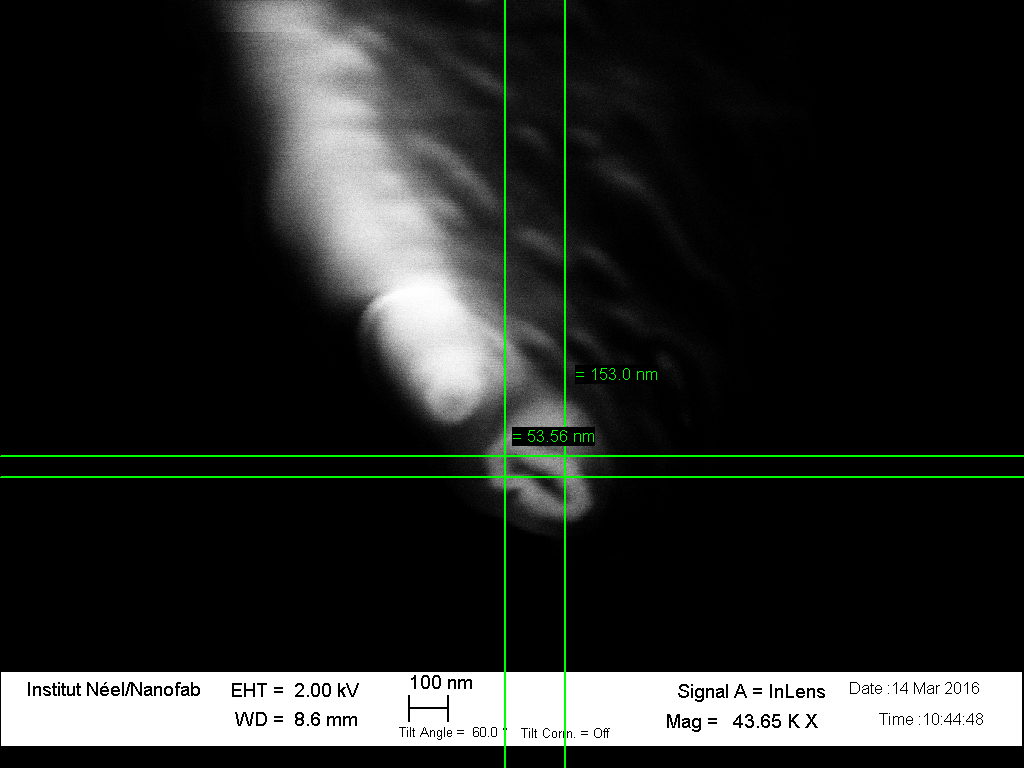
\includegraphics[width=.99\textwidth]{lot33_A1-10.png}
    \caption{Angle $\lambda/2 = 0$}\label{fig:1g}
  \end{subfigure}%
  \begin{subfigure}[b]{.14\linewidth}
    \centering
    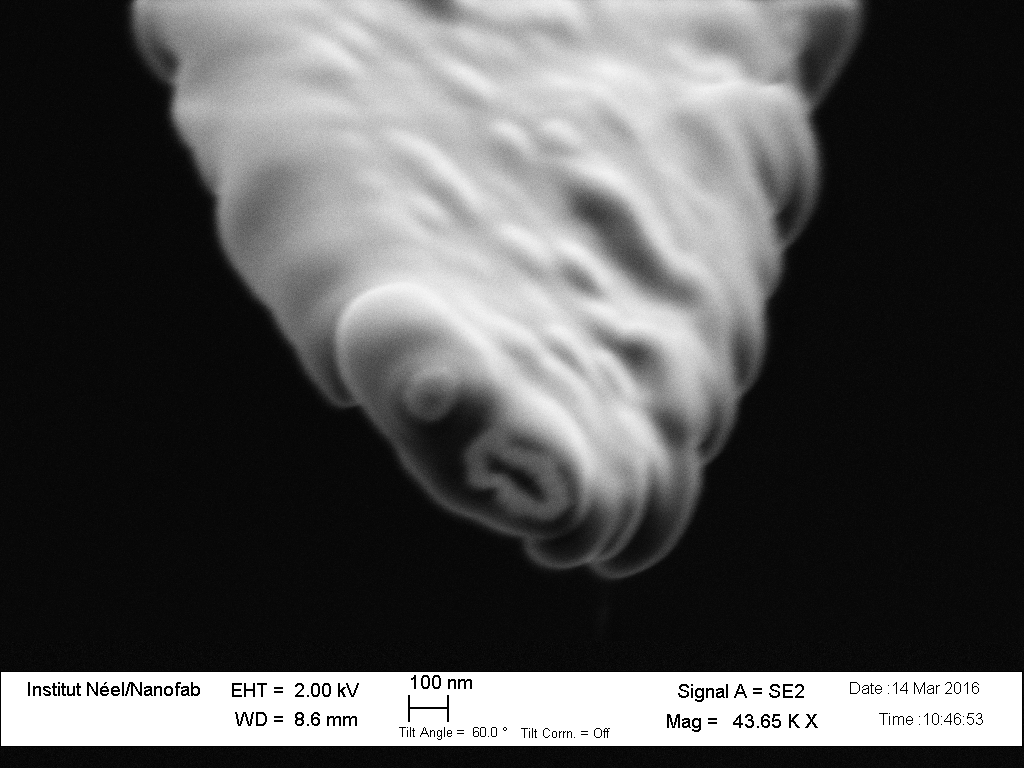
\includegraphics[width=.99\textwidth]{lot33_A1-12.png}
    \caption{Angle $\lambda/2 = 15$}\label{fig:1f}
  \end{subfigure}%
  \begin{subfigure}[b]{.14\linewidth}
    \centering
    \includegraphics[width=.99\textwidth]{lot33_A1.jpg}
    \caption{Angle $\lambda/2 = 30$}\label{fig:1e}
  \end{subfigure}%
  \\
  \vspace{1cm}
  Faible distance ($\simeq 200nm$) :\\
  \vspace{5mm}
  \begin{subfigure}[b]{.14\linewidth}
    \centering
    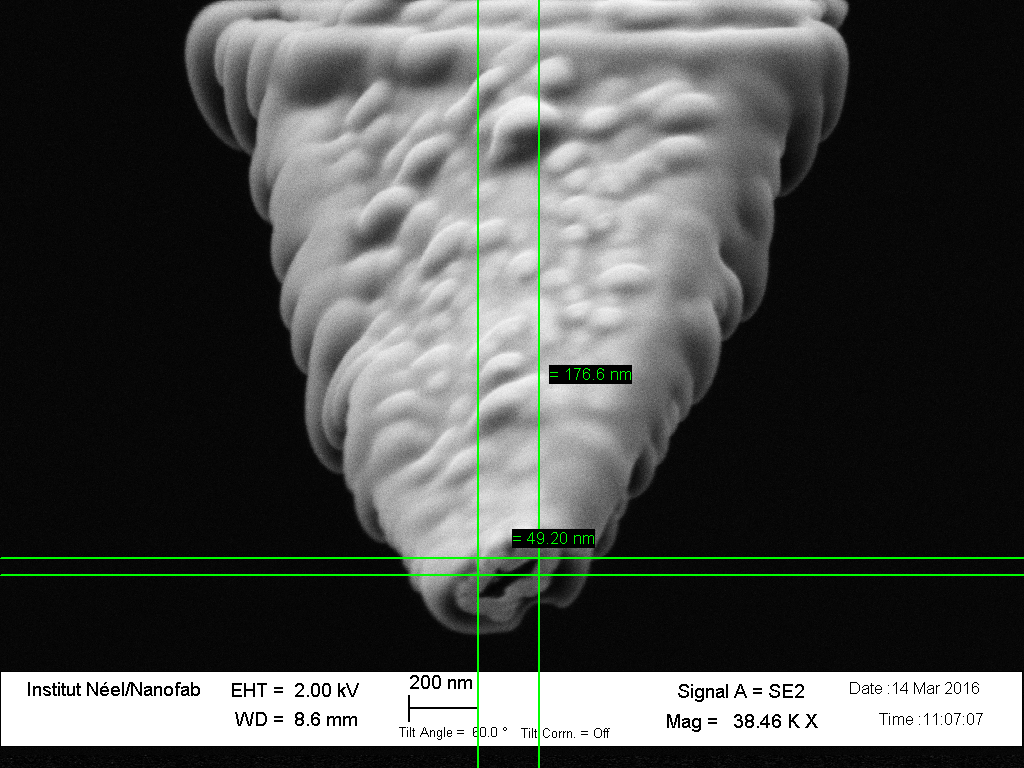
\includegraphics[width=.99\textwidth]{lot33_A362.png}
    \caption{Angle $\lambda/2 = 0$}\label{fig:1g}
  \end{subfigure}%
  \begin{subfigure}[b]{.14\linewidth}
    \centering
    \includegraphics[width=.99\textwidth]{lot33_A363.png}
    \caption{Angle $\lambda/2 = 15$}\label{fig:1f}
  \end{subfigure}%
  \begin{subfigure}[b]{.14\linewidth}
    \centering
    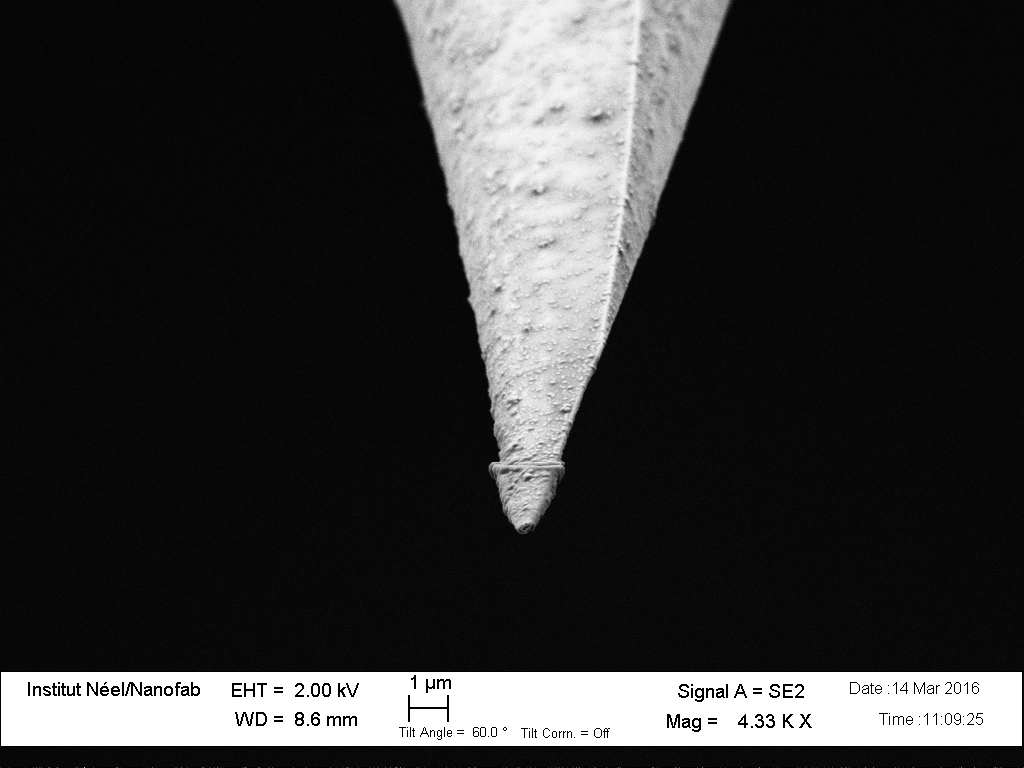
\includegraphics[width=.99\textwidth]{lot33_A366.png}
    \caption{Angle $\lambda/2 = 30$}\label{fig:1e}
  \end{subfigure}%
  \begin{subfigure}[b]{.14\linewidth}
    \centering
    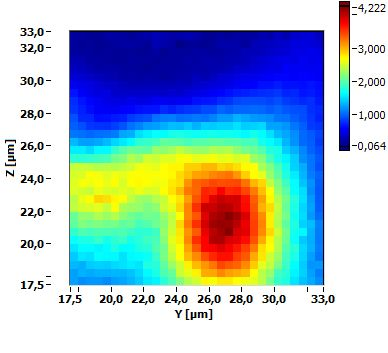
\includegraphics[width=.99\textwidth]{scan_049_g1}
    \caption{Angle $\lambda/2 = 45$}\label{fig:1d}
  \end{subfigure}%   
\end{figure}
\end{document}
